\section{Vorgehen in Regelungstechnik}
Zur Ermöglichung einer strukturierten Vorgehensweise bedarf es einer Orientierung. Dieser Arbeit liegt die in der Vorlesung behandelte Vorgehensweise in der Regelungstechnik zugrunde, welche nachfolgend erläutert wird.

\begin{enumerate}
    \item Detaillierungsgrad für das System festlegen
    \item Physikalisches Modell einschließlich der Störsignale erstellen
    \item Eingangs-, Ausgangs-, Zustands- und Störgrößen des Systems festlegen
    \item Physikalische Einheiten festlegen und ggf. Normierung in Prozent
    \item Analyse des Modells
    \begin{enumerate}
        \item Ruhelagen, Anfangswerte, evtl. Linearisierung nichtlinearer Systeme
        \item Systemeigenschaften ermitteln
    \end{enumerate}
    \item Entwurf
    \begin{enumerate}
        \item Ziele, Arbeitspunkte und Trajektorien festlegen
        \item Entwurf: Struktur, Bereich, Verfahren und Kriterien
    \end{enumerate}
    \item Simulation und Rückinterpretation
\end{enumerate}

\section{Das System}


\subsection{Eigenschaften des Systems}
Wir untersuchen ein System mit Nennergrad 1, einer Totzeit $t$ und einem propoertionalen Übertragungsverhalten. Daraus ergibt sich die Bezeichnung $PT_{1}T_{t}$.

\subsection{Die Übertragungsfunktion}

Formel \ref{eq:G(s)_1} zeigt die Übertragungsfunktion die in diesem Skript analysiert wird. Formel \ref{eq:G(s)_3} zeigt eine etwas andere Darstellung der Formel, sodass die Eigenschaften des Systems leichter abzulesen sind.

\begin{eqnarray}
    \label{eq:G(s)_1}
    G(s) &=& \frac{Y(s)}{U(s)} \\
    \label{eq:G(s)_2}
    &=& \frac{3 * e^{-2s}}{(1+s)} \\
    \label{eq:G(s)_3}
    &=& \frac{3}{1 + s} * e^{-2s}
\end{eqnarray}

\subsection{Eingabe in MATLAB}
Für die Eingabe der Übertragungsfunktion in MATLAB gibt es zwei Möglichkeiten. \\
In manueller Eingabe schreibt man \texttt{G(s) =  3 / (1 + s) * exp(-2 * s)}. \\
In Computer-Algebra wird der Befehl \texttt{sys = tf([3], [1, 1],\textquotedbl IODelay\textquotedbl, 2)} benötigt. Hierbei werden in den beiden Vektoren die Koeffizienten vor $s^0$ bzw. $s^1$ (im Nenner) angegeben. Bei komplizierteren Gleichungen hilft dabei der Befehl \texttt{expand(G(s)}, der einem die benötigten Koeffizienten liefert, was hier jedoch nicht nötig war. Darauf folgt der Befehl \enquote{IODelay}, mit dem die Totzeit $t = 2$ angegeben wird.\\
In beiden Fällen wird in MATLAB damit die Formel \ref{eq:G(s)_3} dargestellt.

\section{Darstellungsformen des Systems}

\subsection{Explizite Darstellung des Übertragungsoperators}

\subsection{Zustandsraumdarstellung}
\subsubsection{Integralgleichung}
\subsubsection{Differentialgleichung}

Die allgemeine Form der Zustandsraumdarstellung lautet:

\begin{align*}
    \dot x & = Ax + Bu \nonumber \\
    y & = Cx + Du
\end{align*}

Für unser System sieht dies folgendermaßen aus:


\begin{subequations}
    \begin{align}
        \dot x & = \begin{bmatrix}
            -1
        \end{bmatrix}x + \begin{bmatrix}
            2
        \end{bmatrix}u \\
        y & = \begin{bmatrix}
            1.5
        \end{bmatrix}x + \begin{bmatrix}
            0
        \end{bmatrix}u
    \end{align}
\end{subequations}

Man kann auch die Zustandsraumdarstellung direkt eingeben, indem man man die Matrizen $A, B, C, D$ belegt und den Befehl \texttt{sys = ss(A, B, C, D)} ausführt. Von hier aus kommt man mit \texttt{tf(sys)} wieder zur Übertragungsfunktion.

Die Zustandsraumdarstellung kann aus der Übertragungsfunktion in einfachen Fällen mit dem Substitutionstrick erstellt werden. Für Systeme, bei denen auch $\dot u, \ddot u, \ldots$ vorkommt, ist das Ganze ein bisschen komplizierter, wird aber in \href{https://de.wikipedia.org/wiki/Zustandsraumdarstellung#Regelungsnormalform}{Wikipedia} beschrieben und kann entsprechend angewendet werden.
Bei sprungfähigen Systemen sieht das noch etwas anders aus und es muss erst eine Polynomdivision gemacht werden, um $d$ zu erhalten. Im Mehrgrößenfall ist es noch komplizierter. (Weiß Hr. Groell auch nicht)

ACHTUNG: Beim Erstellen dieses Dokuments hatte ich zuerst die ANfangswerte vergessen! Das passiert mir in der Klausur nicht, da sonst ein Punkt weg ist !AUSRUFEZEICHEN!11!!1!
Die Anfangswerte werden für die Simulation natürlich benötigt, weil die Funktion wissen muss, wo sie startet.
Die Anfangswerte müssen mit den Anfangswerten der Ein-  Ausgangsdarstellung korrespondieren. 
Das bedeutet $y(0) = CX(0^-) + D(0^-)$

$ \dot y(0^-) = CAx(0^-) + CBu(0^-) + D \dot u (0^-)$

\subsection{Eingangs-Ausgang Differentialgleichung}

Dieses und das folgende Kapitel sind bei meinen Mitschrieben als 3a und 3b zusammengefasst

\begin{eqnarray*}
    G(s) =\frac{Y(s)}{U(s)} &=& \frac{6s^2 - 5s + 1}{120s^3 + 74s^2 + 15s +1} \\
    Y(s)(120s^3 + 74s^2 + 15s +1) &=& U(s) (6s^2 - 5s + 1) \\
    120 \dddot y + 74 \ddot y + 15 \dot y &=& 6 \ddot u + 5 \dot u + u
\end{eqnarray*}

\subsection{Übertragungsfunktion}
Entweder wir streichen das erste kapitel und schreiben hier den Kram hin, oder iwie doppelt, oder ne andere Lösung -> Theresa ist gefragt!

\subsection{Gewichtsfunktion g(t) (Impulsantwort)}
Dieses und das folgende Kapitel sind bei meinen Mitschrieben als 4a und 4b zusammengefasst


In Abbildung \ref{fig:impuls} ist die Reaktion des Systems auf technischen Eingangssprung zu sehen.
\\
In MATLAB lässt sich das mit dem Befehl \texttt{impulse(sys)} simulieren, wodurch man die numerische Lösung erhält. In MATLAB lässt sich das mit dem Befehl \texttt{step(sys)} simulieren, wodurch man die numerische Lösung erhält. Die Übergangsfunktionfunktion $h(t)$ lässt sich aber auch analytisch berechnen und man erhält die explizite Lösung. Hierbei hilft einem der Befehl \texttt{ilaplace()}, der die Laplace-Transformierte zurückliefert:
\begin{lstlisting}
    syms g(t)
    g(t) = ilaplace(H(s))
    t = [0:0.1:8]
    plot(t, g(t))
\end{lstlisting}

Beide Befehle führen zum folgenden Graphen:



\begin{figure}[H]
    \label{fig:impuls}
    \centering
    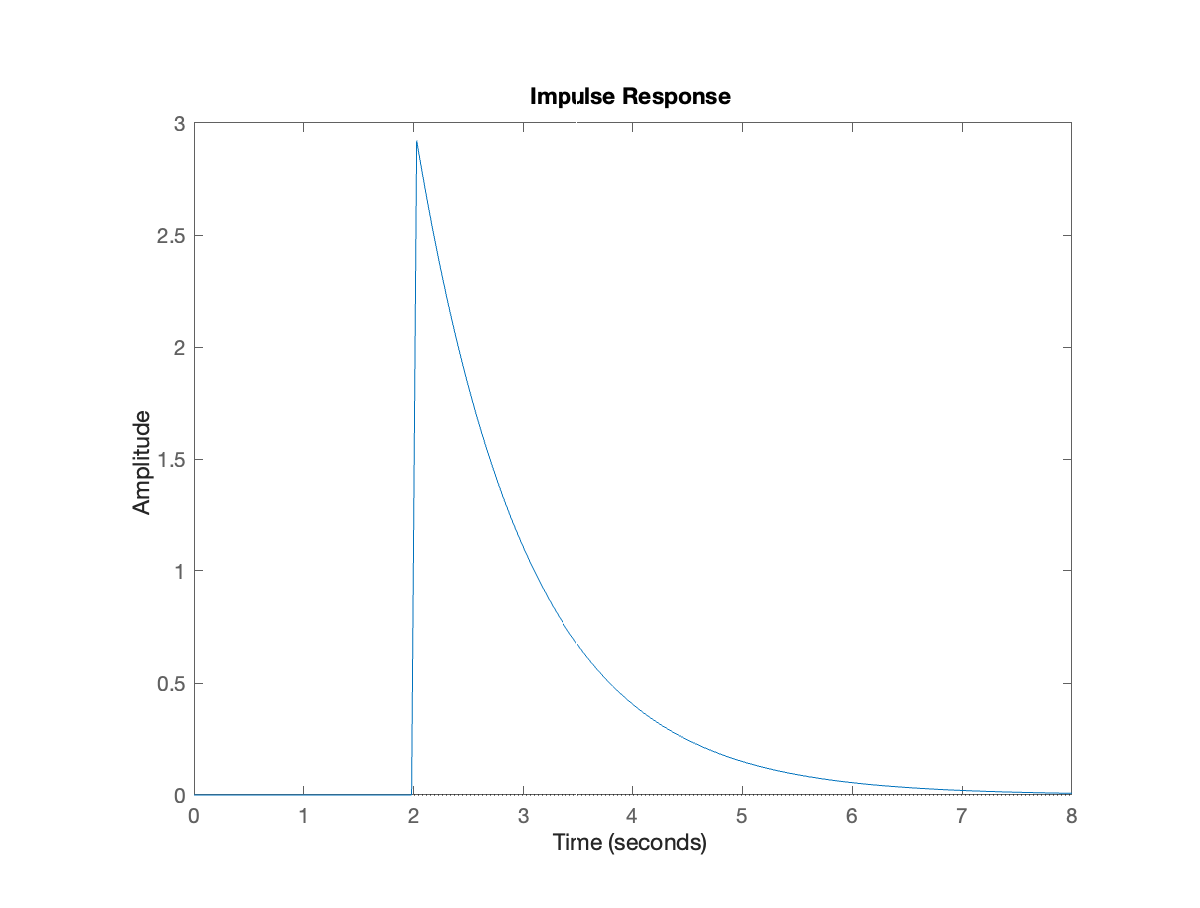
\includegraphics[width=0.8\textwidth]{Bilder/ImpulsAntwortPT1Tt.eps}
    \caption{Impulsantwort}
 \end{figure}



\subsection{Übergangsfunktion h(t) (Sprungantwort)}

In Abbildung \ref{fig:sprung} ist die Reaktion des Systems auf den Heaviside-Funktion zu sehen. Diese ist wie folgt definiert:

\[
\sigma (t) = \begin{cases} 0 & \text{für t < 0} \\ 1 & \text{für t > 0} \end{cases}  
\]
\\
In MATLAB lässt sich das mit dem Befehl \texttt{step(sys)} simulieren, wodurch man die numerische Lösung erhält. Die Übergangsfunktionfunktion $h(t)$ lässt sich aber auch analytisch berechnen und man erhält die explizite Lösung. Hierbei hilft einem der Befehl \texttt{ilaplace()}, der die Laplace-Transformierte zurückliefert:

\begin{lstlisting}
    H(s) = G(s) / s
    syms h(t)
    h(t) = ilaplace(H(s))
    t = [0:0.1:8]
    plot(t, h(t))
\end{lstlisting} 

Beide Befehle führen zum folgenden Graphen:

\begin{figure}[H]
    \label{fig:sprung}
    \centering
    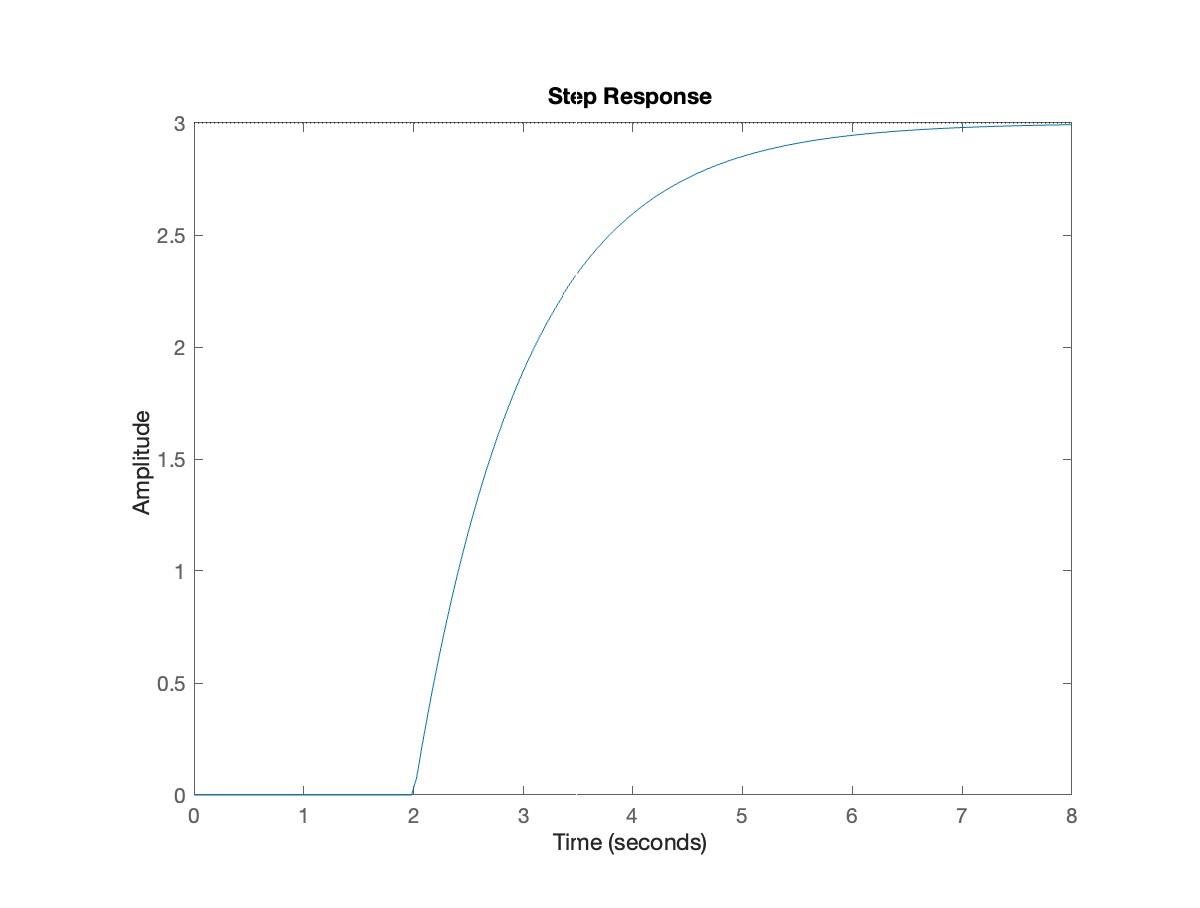
\includegraphics[width=0.8\textwidth]{Bilder/SprungantwortPT1Tt.eps}
    \caption{Sprungantwort}
 \end{figure}


\subsection{Frequenzgang ($G(j * \omega)$)}
Dieses und die folgenden Kapitel sind in meinen Mitschrieben als 5a, 5b und 5c zusammengefasst.

Zum Frequenzgang $G(j * \omega)$ gelangt man, indem man in $G(s)$ das $s$ durch $j * \omega$ ersetzt.

Das bedeutet, das für jede Frequzenz $\omega$ eine komplexe Zahl $j$ mit Real- und Imaginärteil oder mit Betrag und Phase darstellt.

\subsection{Ortskurve(Nyquist-Plot)}
Im Nyquist-Plot wird der über $\omega$ parametrisierte Frequenzgang als Kurver in der komplexen Ebene mit Real- und Imaginärteil dargestellt.
MATLAB bietet hier den Befehl \texttt{nyquist(sys)} an, welche zum folgenden \hyperref[fig:nyquist]{Plot} führt. Dabei zeigt MATLAB die Kurve von $-\infty$ bis $+\infty$ an, was in unserem Beispiel jedoch nicht nötig ist.

\begin{figure}[H]
    \label{fig:nyquist}
    \centering
    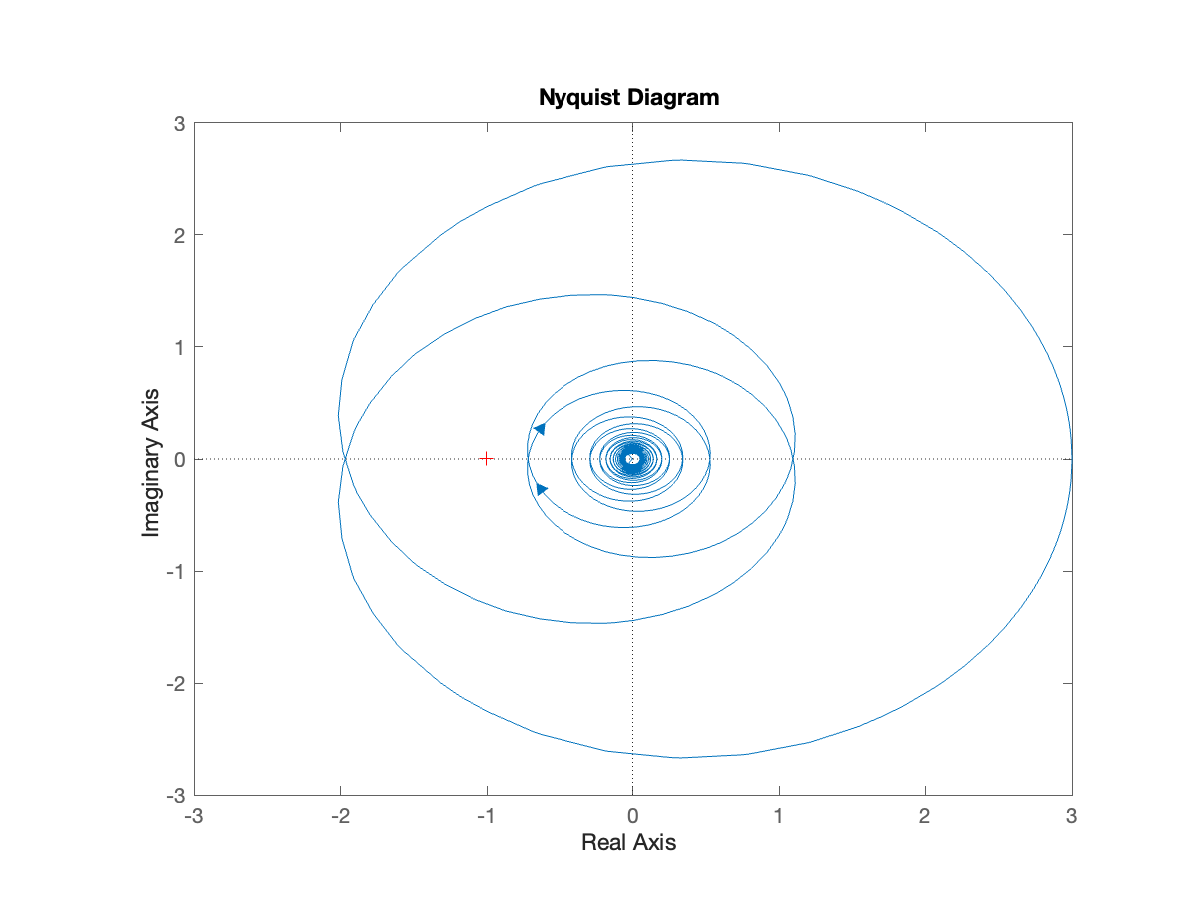
\includegraphics[width=0.8\textwidth]{Bilder/NyquistPT1Tt.eps}
    \caption{Nyquist-Plot}
 \end{figure}

 Darüber hinaus ist es in MATLAB möglich, mit dem Cursor entlang der Kurve zu gehen, um sich einzelne Werte genauer anzuschauen, wie in \autoref{fig:nyquistCursor} dargestellt.

 \begin{figure}[H]
    \label{fig:nyquistCursor}
    \centering
    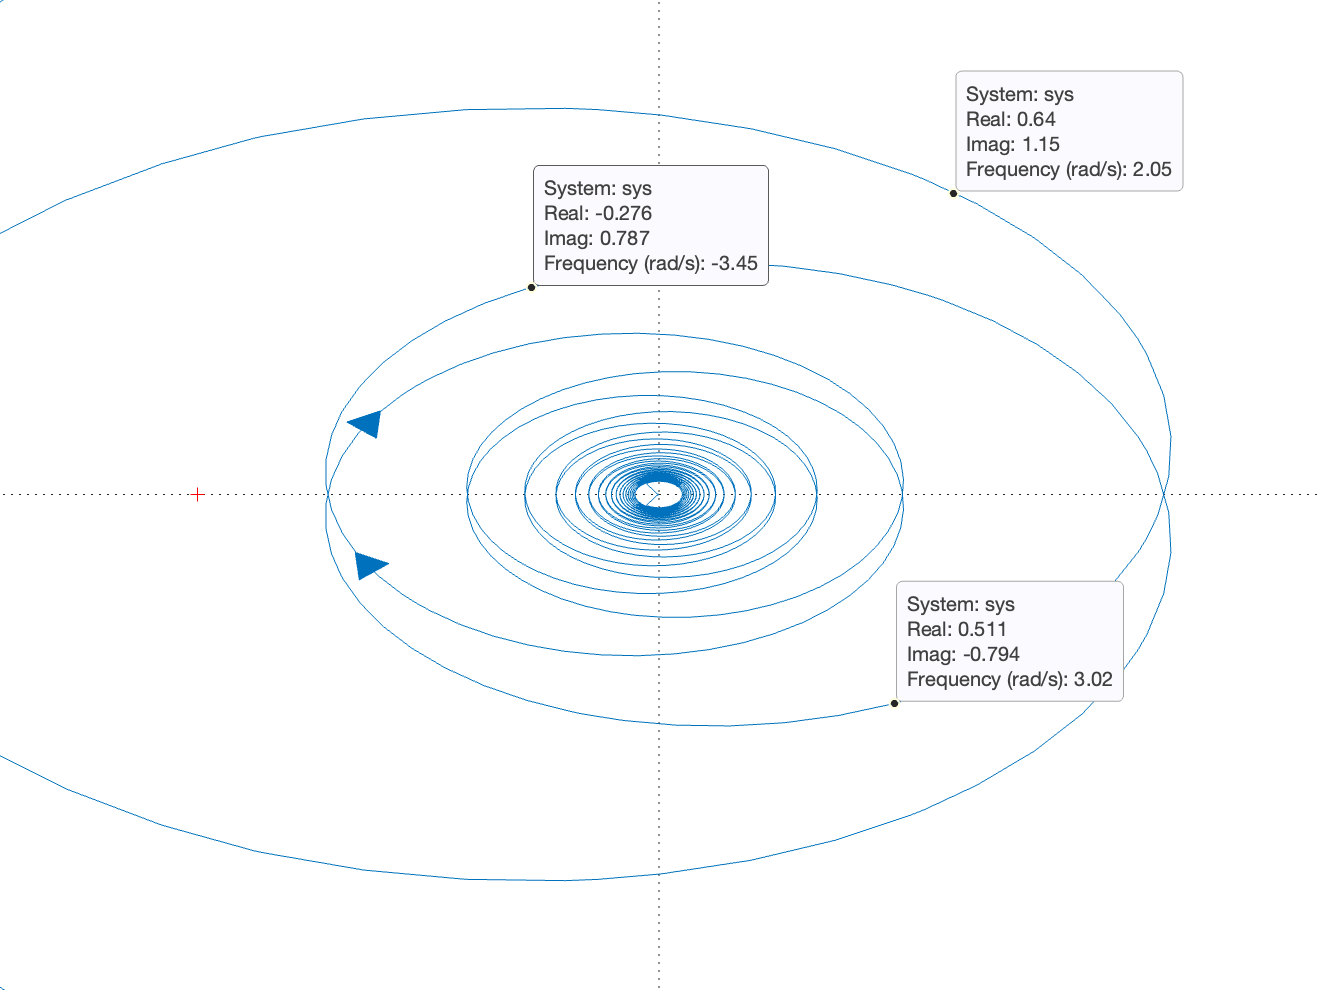
\includegraphics[width=0.8\textwidth]{Bilder/NyquistCursorPT1Tt.png}
    \caption{Screenshot: Informationen im Nyquist-Plot}
 \end{figure}

 Systemtheoretisch entspricht der Frequenzgang einem Schnitt der komplexen Funktion $G(s)$ entlang der imaginären Achse: $G(s)\Bigr\rvert_{s = j * \omega}$

\subsection{Bode-Diagramm}
Im Bode-Diagramm sind der Betrag des Frequenzgangs über $\omega$ in Dezibel(dB) und die Phase des Frequenzgangs über $\omega$ in Grad($^\circ$) dargestellt. Damit die Kurven schön aussehen, verwendet MATLAB eine doppelt logarithmische Darstellung. Der dazugehörige MATLAB-Befehl ist \texttt{bode(sys)}. Streng genommen wird in MATLAB im oberen Bild die Amplitudenverstärkung angzeigt, die ein Sinus-Signal stationär erfährt (bei Eigenwert = 1), währenddessen im unteren Bild die Phasenverstärkung zu sehen ist.

\begin{figure}[H]
    \label{fig:bode}
    \centering
    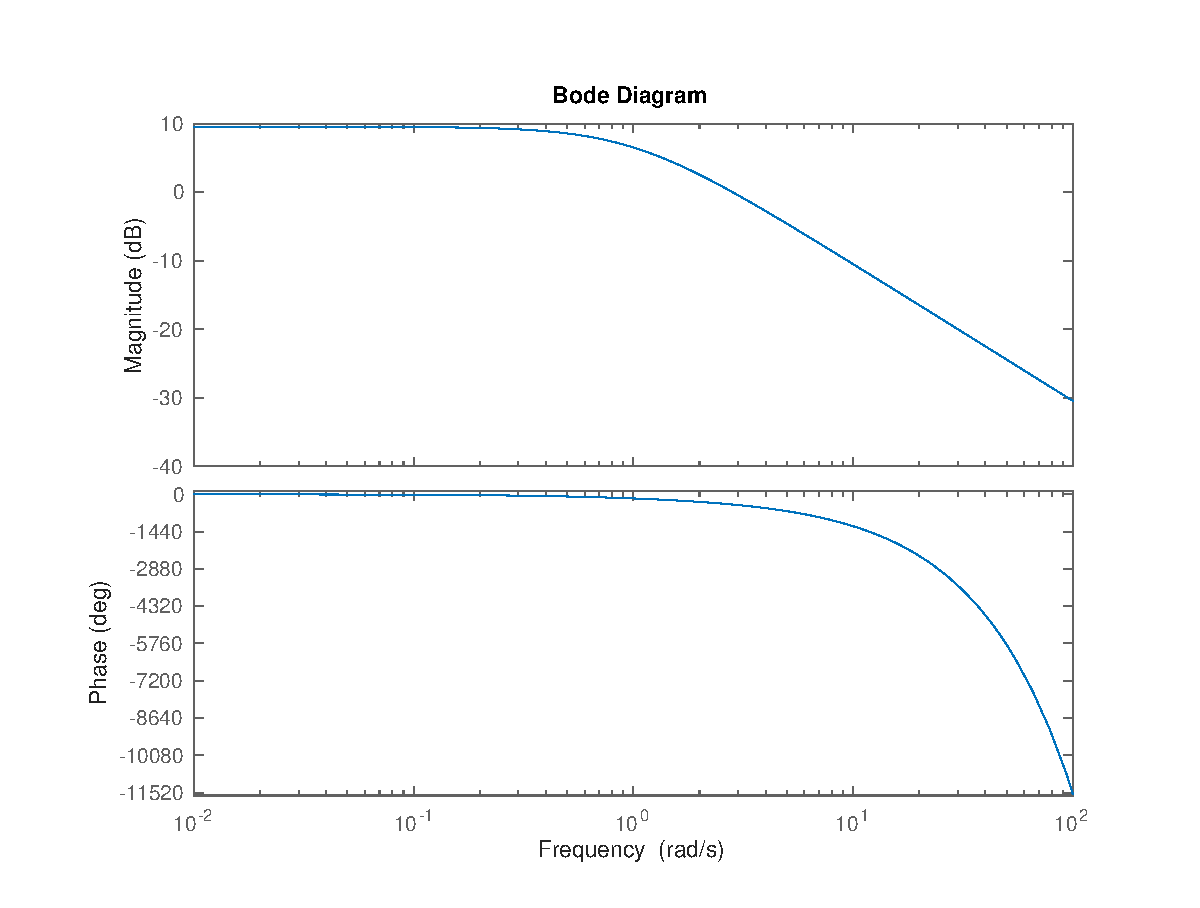
\includegraphics[width=0.8\textwidth]{Bilder/BodePT1Tt.eps}
    \caption{Bode-Plot}
 \end{figure}

\subsection{Statische Kennlinie}
Keine Ahnung

\subsection{Pol-Nulstellen-Plot}
\autoref{fig:poleZero} zeigt den Pol-Nulstellen-Plot zu unserem System. Der passende MATLAB-Befehl hierfür lautet \texttt{pzplot(sys)}. MATLAB markiert mit \textbf{o} die Nullstellen und mit \textbf{x} die Polstellen des Systems. In unserem Beispiel hat das System aber keine Nulstellen, da der Zählergrad 0 ist, weshalb in der Abbildung kein \textbf{o} zu sehen ist. Da der Nenner unseres Systems aber den Grad 1 mit $1 + s$ ist, hat unserer System eine reale Polstelle bei s = -1, was in der Abbildung mit den \textbf{x} gekennzeichnet ist.

\begin{figure}[H]
    \label{fig:poleZero}
    \centering
    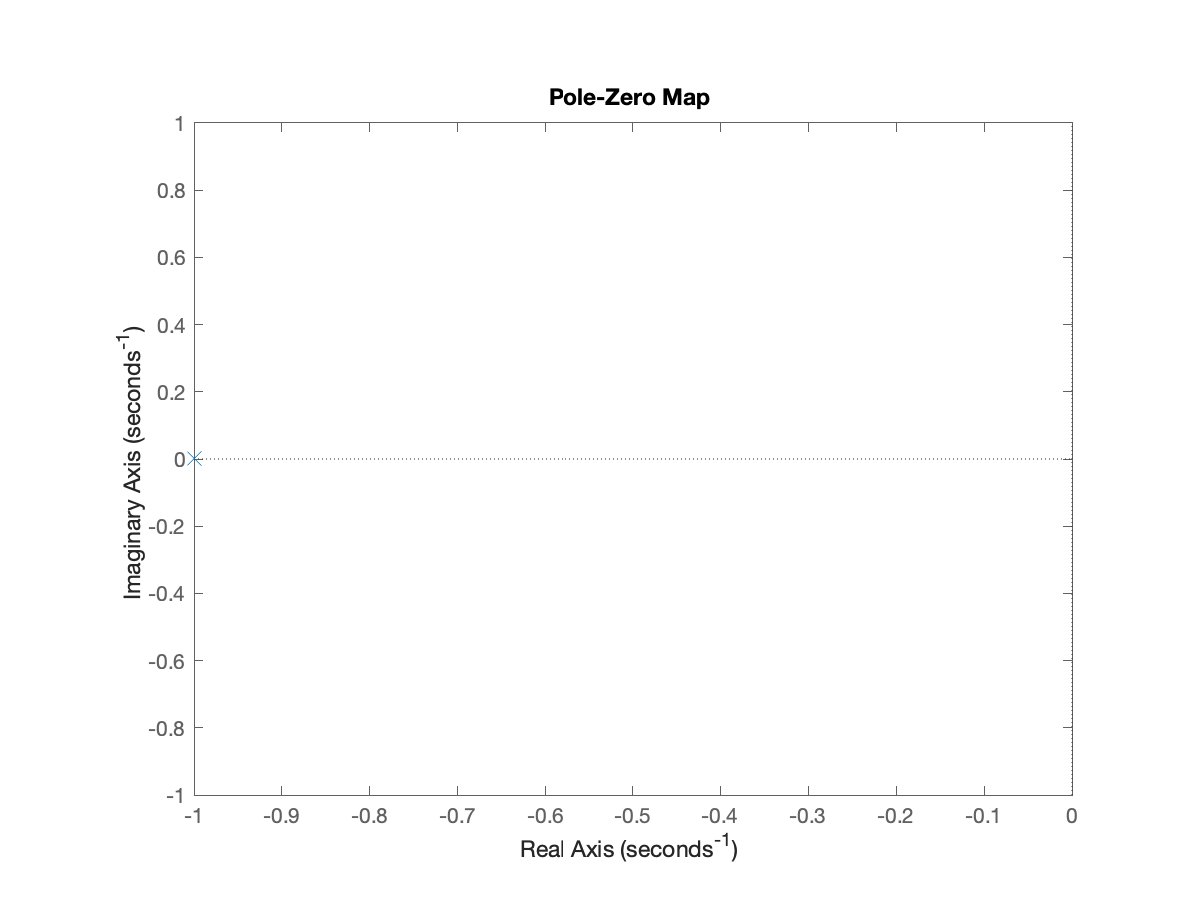
\includegraphics[width=0.8\textwidth]{Bilder/PoleZeroPT1Tt.eps}
    \caption{Bode-Plot}
 \end{figure}
